\documentclass[12pt]{article}
\usepackage[latin1]{inputenc}
\usepackage{graphicx,subfigure}
\topmargin -1mm
\oddsidemargin -1mm
\evensidemargin -1mm
\textwidth 155mm
\textheight 220mm
\parskip 2mm
\parindent 3mm
%\pagestyle{empty}


\begin{document}

\begin{center}

{\Large \bf Step Map and Plot (SMP) in Open Calphad (OC)}

{\large Basic description and documentation}

Bo Sundman, \today

\end{center}

The work on the step, map and plot procedures is progressing slowly.
The main work started late in 2013 and we are now at the end of
September 2014.  Serious errors in the other parts of the software
have also been found and corrected.  So it is interesting to show that
even if the software as a whole becomes better, some calculations were
better without all the bugfixes.  In Fig.~\ref{fg:hss} two isopleths
of a high speed steel (I think the composition is slightly different)
are shown, one calculated in May 2014 and the other in October.  The
one from May is clearly better but at that time there were many bugs
that had been eliminated in October.  So evidently some bugs
compensate each other.
\begin{figure}[!h]
\includegraphics[width=50mm,angle=-90]{figs/oc-hss-140513.ps}
\includegraphics[width=50mm,angle=-90]{figs/oc-hss-141002.ps}
\caption{Figures showing progress sometimes goes backwards.  The left
  hand figure was calculated in May 2014 (before there was a date on
  the diagrams) and the right in October with several missing lines.
  Considering all the errors that has been found in the minimizer and
  other parts of the OC software it is remarkable it was possible to
  calculate anything in May.}\label{fg:hss}
\end{figure}

\end{document}
